%&pdflatex --translate-file=cp1250pl

\documentclass[10pt]{article}

\usepackage[pdftex]{graphicx}
\graphicspath{{./pdf/}}

\usepackage{amsmath} \allowdisplaybreaks
\usepackage{amssymb}
\usepackage{moreverb}
\usepackage{metalogo}

\usepackage{csagh}

\usepackage{polski}
\renewcommand\figurename {Figure}
\renewcommand\tablename  {Table}
\renewcommand\refname    {References}

\def\listingoffset{\leftmargini}
\def\listinglabel#1{\rlap{\footnotesize\sffamily\the#1}%
    \hskip\listingoffset{}\relax}

\def\preTeXt{\textsf{pre\kern-1pt\textbf{\TeX}t}}


\makeatletter
\newcounter{@xample}
\def\the@xample{\arabic{@xample}}
\def\theorem@headerfont{\normalfont\bfseries\sffamily}
\def\nam@example{Example}
\newenvironment{example}{\refstepcounter{@xample}%
  \begin{trivlist}\normalfont\rmfamily
  \item[\hskip\labelsep%
        \theorem@headerfont\nam@example\space\the@xample.\space]\space}
 {\end{trivlist}}
\newenvironment{example*}{
  \begin{trivlist}\normalfont\rmfamily
  \item[\hskip\labelsep%
        \theorem@headerfont\nam@example.\space]\space}
 {\end{trivlist}}
\makeatother


\begin{document}

\begin{opening}

\title{Preparing publications\newline
    for ``Computer Science'' annual}

\author[preTeXt,
         \URL{http://www.pretext.com.pl},
         e-mail: \URL{jk@pretext.com.pl}]
       {Jacek Kmiecik}

\date{Krak�w, 29.11.2014}

\begin{abstract}
  In this paper we present a~short instruction for preparing
  manuscripts for ,,Computer Science'' annual with the use of
  \LaTeX{} and the \texttt{csagh.sty} style.
\end{abstract}

\keywords{\LaTeX, ``Computer Science'', AGH Publishing House}
\end{opening}


\section{Introduction}

The task of the \texttt{csagh.sty} style
is to enable prospective authors to prepare
articles to ,,Computer Science'' journal
according to a~typographical template and the editorial rules
adopted by the AGH University of Science and Technology Publishing House.
Present paper aims at the presentation of ways of
using this style, as well as the facilitation 
of the usage of the other packages, which could be 
necessary to set the specific contents of some articles.

It has been assumed that every author has full freedom to use
any package dedicated to the \LaTeXe{} format ---
while preparing the \texttt{csagh.sty} style, efforts have been made
to assure that it would not conflict with other styles (packages),
which acquired compatibility with the currently distributed
\TeX  and \LaTeXe installations.\footnote{It has been assumed that
compilation will be made using pdf\LaTeX and the package was tested
from this point of view. However, there is no guarantee that inclusion
of any package or group of packages will not cause conflicts
during the document processing. Similarly, usage of the \XeLaTeX{} compiler
may yield unexpected results in some malicious cases.}
Discussed style defines proper column sizes, enables to choose proper
language of an article (appropriate patterns of words hyphenation,
characteristic document structures names etc.), to format titles
and headings, structures of type: definition, theorem, proof etc.,
to describe in proper way: figures and tables, 
and required article components, such as:

%
\begin{itemize}
\item[1)] an article title in English,
\item[2)] an abstract (max 250~words),  
\item[3)] a~set of keywords in English.
\end{itemize}

Prepared author's typesetting composes a~basis for further
editorial works, adjustments, proofs, pagings --- in order to 
enter afterwards into the composition of publication of the next annual
together with the other articles. Pagination, live pagination,
colophon, table of contents and remaining elements of finished publication are added
during this phase.

All of the packages used within the style, i.e.:
\texttt{ifthen.sty},
\texttt{exscale.sty},
\texttt{array.sty},
\texttt{theorem.sty} ---~come from the standard distribution
\LaTeXe and are essential for proper functioning of the discussed style.

Both \texttt{csagh.sty} file and remaining sample and documentation files
are distributed on a~basis of the free software (GPL licence), made available 
free of charge to concerned\footnote{E.g. from sites \texttt{http:/\kern-2pt/www.wydawnictwoagh.pl}
--- of the AGH University of Science and Technology Publishers.}.
With formal regards, the author of the present paper is entitled to
copyrights of \texttt{csagh.sty} package \TeX code.
Any remarks concerning the functioning of macros, way of using them
or noticed errors --- please direct to an e-mail address: 
\texttt{jk@pretext.com.pl}.


\section{Document structure}

Document structure would not be anything new for a~person
familiar with creating the \LaTeXe{} documents. I refer people concerned with
studying the whole \TeX-nology more closely to the specialist literature
or to the Internet resources rich in this subject matter.

Below there is a~listing presenting the first lines of \LaTeX{} file
which serves to prepare article for the ,,Computer Science'' annual.

\medskip
\begin{listing}[1]{1}
%&platex --translate-file=cp1250pl
\documentclass[10pt]{article}
\usepackage{amsmath}
\usepackage{amssymb}
\usepackage{moreverb}
\usepackage[dvips]{graphicx}
\graphicspath{{./pdf/}}
\usepackage{csagh}
\begin{document}
... [an essential content of an article] ...
\end{document}
\end{listing}
\medskip

\begin{description}
\item[Line 1] --- the first line of the main document file,
		beginning from the first column; this line has
		a special meaning in modern \TeX distributions
		(so-called \textit{web2c}): it informs a~compiler about
		used document processing format (here: \verb|&platex| means
		Polish LaTeX format) and characters encoding methods adopted
		in the  document (here: \verb|--translate-file=cp1250pl| means
		Windows code page);
\item[Line 2] --- a~choice of the appropriate class of the
		article being composed; in this case
		it is the \verb|article| class which enables typesetting
		with the use of the 10 pt Computer Modern font type;
\item[Lines 3 and 4] --- additional packages which enable to compose
		advanced mathematics, with the use of the characters and symbols
		unavailable in the basic \LaTeX macros set
    \cite{AMS:doc};
\item[Line 5] --- the additional package for composing samples
		of programs code with the use of the so-called machine text,
		with the possibility of the code lines numbering\footnote{\LaTeX has
		inner environments of the machine typesetting 
    \texttt{verbatim} and \texttt{verbatim*} --- nevertheless, in many cases
		it is necessary to use much more expanded environments. There is the
		\texttt{moreverb} package used in the present article.};
\item[Lines 6 and 7] --- the additional package which enables to include
		graphics in the PDF;
    \verb|\graphicspath| command enables to indicate a~directory
		where the figures used in the paper are kept;
\item[Line 8] --- \verb|\usepackage{csagh}| is exactly the discussed
		package (style) for composing articles of the
    ,,Computer Science'' annual;
\item[Lines 9--11] --- the \verb|{document}| environment is a~place
		where an essential content of the article would be created.
\end{description}

All lines of the \LaTeX code, placed before the \verb|{document}|
environment, are named as a~\textit{document preamble}.
There we have a~possibility to include all additional packages
which may be needed for a~given article composing.

In the distribution of the \texttt{csagh} package 
there is a~sample file (\textit{template}), which
may be used to begin work on an own document.

In the further part of the paper there is an overview of the elements included
in the \verb|{document}| environment.


\section{How to get started?}

The assumptions of the ,,Computer Science'' drafting committee determine
that a~content of an article may be written in Polish or in English.
Regardless of the language version, each article should own a~title, an abstract
and keywords in both languages. It is also required that author (or authors)
provides exact affiliations: a~name and an address of the institution
and a~contact address.

All of these pieces of information are written into the specially
prepared \verb|{opening}| enviornment, by means of the appropriate macros:

\medskip
\begin{listing}[1]{1}
\begin{opening}
 \title{Preparing publications\newline
    for ``Computer Science'' annual}
 \author[\textsf{pre\kern-1pt\textbf{\TeX}t},
         \URL{http://www.pretext.com.pl},
         e-mail: \URL{jk@pretext.com.pl}]
        {Jacek Kmiecik}
 \date{Krak�w, 3\textsuperscript(rd) July 2004}
 \begin{abstract}
  In this paper we present a~short instruction for preparing
  manuscripts for ,,Computer Science'' annual with the use of
  \LaTeX{} and the \texttt{csagh.sty} style.
 \end{abstract}
 \keywords{\LaTeX, ``Computer Science'', AGH Publishing House}
\end{opening}
...
...
\end{document}
\end{listing}
\medskip

A content of the \verb|{opening}| enviornment is composed as
an article's beginning taking proper order and the way of formatting
under consideration. An order of particular pieces of information
depends on the adopted language version, chosen as the package option.
In case of an absence of any of these elements, a~suitable message is shown. So:

\begin{description}
\item[\texttt{\string\author\string{...\string}}]
    --- contains information about the author or the authors of the article,
    together with particular affiliations
    (the third line of the code presented above);
    alternatively macro called
    \texttt{\string\autor\string{...\string}} may be used;
\item[\texttt{[...]}]
    --- contains information about the institution of the author (authors)
    of the article, together with contact addresses;
    in case of many authors and/or different affiliations, it is possible
		to apply the trick:

\medskip
\begin{listing}[1]{1}
\author[Institution, address, the first author's e-mail address]{Author-1}
\author[Institution, address, the second author's e-mail address]{Author-2}
\autor{Author-3} % the third author will have the last affiliation
                 % assigned, that is identical to the second author's
\author[Institution1, address1, the fourth author's e-mail address1,
        Institution2, address2, the fourth author's e-mail address2,]{Author-4}
\end{listing}
\medskip

   -- an absence of the affiliation next to the Author (an absence of an optional parameter in the
   \verb|\author| command) causes an assignment of the affiliation of the previous Author 
   (if this situation happens next to the first Author, an error message is shown).

\item[\texttt{\string\title\string{...\string}}]
    --- a~title of the article;
\item[\texttt{\string\keywords\string{...\string}}]
    --- a~set of the keywords;
\item[the \texttt{abstract} environment]
    --- an abstract of the article (max 250 words);
\item[\texttt{\string\date\string{...\string}}]
    --- a~date of the article submission to the Editorial Board; optional
    information (the item may not appear at all).
\end{description}


\section{Document structure}

\subsection{A logical section of the document's content}

An exemplary article, comprising logically coherent discussion
of a~given subject, should be divided thematically into parts.
These logical fragments are usually called the subsections
and have an appropriate ordinal number and a~title assigned.

Five-level nesting of consecutive subsections is adopted in
the present template. The first three subsections will be provided with
an ordinal numbering, i.e.:
\verb|\section{...}|,
\verb|\subsection{...}|,
\verb|\subsubsection{...}|.
Last two levels of the nesting ---
\verb|\paragraph{...}| and~%
\verb|\subparagraph{...}|,
will be identified in the text with another font type only.

A numbering of the particular units is made automatically.
The Author may perform a~change of the level of the subtitles numbering
by himself, by using the instruction in the document preamble:

\begin{listing}[10]{2}
\setcounter{secnumdepth}{3}
\end{listing}

\noindent
--- the record above declares a~three-level subtitles numbering.


\subsection{Enumerations}

\LaTeX{} provides three environments for enumerations creation:
%
\begin{enumerate}
\item \verb|itemize|,
\item \verb|enumerate|,
\item \verb|description|.
\end{enumerate}
%
In each of these three enviornments, new enumeration element
begins with the \verb|\item| command, which may contain an
optional parameter put in the square brackets. Lists of numbered
elements are created with the use of the \verb|enumerate| environment.
For instance:
%
\medskip
\begin{listing}[1]{1}
\begin{enumerate}
 \item itemize,
 \item enumerate,
 \item description.
\end{enumerate}
\end{listing}
\medskip

There are some rules concerning
the creation of lists:
%
\begin{itemize}
\item Each enumeration element begins with a~label. The label
    in the present enumeration (the \verb|itemize| environment)
		is a~black ,,bullet'' type dot.
\item Lists may be nested one in another:
    \begin{enumerate}
    \item Labels in the \verb|enumerate| enumerations are numbers
        or letters.
    \item \LaTeX{} uses arabic numerals in this environment's
        enumerations by default.
    \item Label's separator is a~dot.
   \end{enumerate}
    \LaTeX{} enables to nest the \verb|itemize| enumeration environments
    four times, what is usually completely sufficient.
		A deeper nesting may make text reading and comprehension
		more difficult.
\item Empty lines between enumeration elements do not have
		any meaning. They form the next paragraph of the text
		in the current enumeration point.
\item[(!)] Labels of \verb|itemize| environment may be defined
    manually, by providing an optional parameter in the
    \verb|\item| command, i.e. in the current \verb|\item[(!)]| point.
\end{itemize}

Labels of the consecutive items in the \verb|description| environment
are defined, using exactly the optional parameter of the
\verb|\item| command. Although this parameter is optional,
its absence may produce a~strange result in the finished setting.

There is an example of the \verb|description| environment usage:
%
\begin{description}
\item[Antiqua] is a~type of a~latin alphabet print script
   deriving from the humanistic handwriting.
\item[Cyrillic script] the Slavic alphabetical script consisting of
   43 letters patterned on the shapes of the Greek uncial script
   from the IX century.
\item[Script typeface] a~kind of a~print script imitating
   handwriting made with various utensils: pen, stick,
   brush etc. usually slanted to the right
   (selection based on \cite{AT:lpd}).
\end{description}
%
and \LaTeX{} code fragment for this part of the article setting:
%
\medskip
\begin{listing}[1]{1}
\begin{description}
 \item[Antiqua] is a~type of a~latin alphabet print script ...
 \item[Cyrillic script] the Slavic alphabetical script ...
 \item[Script typeface] a~kind of a~print script ...
 ...
\end{description}
\end{listing}
\medskip


\subsection{Mathematical formulas}

The mathematical formulas setting --- this is the real strength of the \LaTeX
(the \TeX basically). Modern computer programs stay far behind within this scope
for ages (for 25 years exactly!), as they offer a~meagre substitute of the
provisional mathematical symbols setting at most.

Inter-paragraph mathematical formulas are composed inside
the dollar signs \verb|$...$| or inside \verb|\(|
and \verb|\)| commands. For example, \verb|$e=mc^2$|
or \verb|\(e=mc^2\)| records produce the equation: $e=mc^2$.
\LaTeX{} treats a~formula as a~word, which may be
divided between lines in some places only. Spaces
before \verb|\(| and after \verb|\)| are treated as normal
spaces between words.

If mathematical formula is too long, it may be exposed with the use of
\verb|$$...$$| command, to fit it aesthetically within the text.
For instance, the formula:
%
$$
  e=mc^2
$$
%
has been obtained by means of \verb|$$e=mc^2$$| command.\vadjust{\goodbreak}

If it is necessary to assign an ordinal number to a~formula,
in order to refer to it later ---
we use so-called exposed formulas. Canonical \LaTeX{}
provides the \verb|displaymath|, the \verb|equation|
and the \verb|eqnarray| environments, to compose such formulas.
The \verb|displaymath| and \verb|equation| environments are identical, except that
the \verb|equation| adds a~consecutive ordinal number to the formula.
Commands \verb|\[| and \verb|\]| are synonyms of the \verb|displaymath| environment.
\verb|Eqnarray| environment consists of exposed multiline numbered formulas.
Its variety is a~,,star'' version \verb|eqnarray*|, which do not
number consecutive lines of a~formula.


\subsection{When LaTeX fails, that is very advanced mathematics}

Unfortunately, the practice has revealed that the environments and
the mathematical commands provided by the canonical \LaTeX are too meagre
to compose very complex mathematical formulas. Therefore, special
packages providing additional environments with
greater possibilities of formulas paging and with an access
to bigger amount of symbols and signs have been created
to facilitate the authors' work. Such a~commendable and fully
compatible with \LaTeX package is the \AmS-\TeX.

For instance, \eqref{eq:gather1} and \eqref{eq:gather2} formulas
composed with the \verb|gather| environment:
%
\begin{gather}
 a~= a_1 + b_1 - c_1
  \label{eq:gather1}\\
 b = a_2 + b_2 - c_2 - d_2 + e_2
 \label{eq:gather2}
\end{gather}

\begin{listing}[1]{1}
\begin{gather}
 a~= a_1 + b_1 - c_1
  \label{eq:gather1}\\
 b = a_2 + b_2 - c_2 - d_2 + e_2
 \label{eq:gather2}
\end{gather}
\end{listing}
\medskip
%
\eqref{eq:split} formula composed with the \verb|split| environment:
%
\begin{equation}\label{eq:split}
\begin{split}
    a~& = b + c + d + e + f + g + h + i + j + k + l + m -\\
      &\quad - n + o - p + q - r + s - t + u - v + w =\\
      & = x + y =\\
      & = z
\end{split}
\end{equation}

\begin{listing}[1]{1}
\begin{equation}\label{eq:split}
\begin{split}
    a~& = b + c + d + e + f + g + h + i + j + k + l + m -\\
      &\quad - n + o - p + q - r + s - t + u - v + w =\\
      & = x + y =\\
      & = z
\end{split}
\end{equation}
\end{listing}
\medskip
%
or \eqref{eq:align1} and \eqref{eq:align2}
composed with the \verb|align| environment:
%
\begin{align}
  a_{11} &= b_{11}        & a_{12} &= b_{12}       \label{eq:align1}\\
  a_{21} &= b_{21}+c_{21} & a_{22} &= b_{22}+c_{22}\label{eq:align2}
\end{align}

\begin{listing}[1]{1}
\begin{align}
  a_{11} &= b_{11}        & a_{12} &= b_{12}       \label{eq:align1}\\
  a_{21} &= b_{21}+c_{21} & a_{22} &= b_{22}+c_{22}\label{eq:align2}
\end{align}
\end{listing}
\medskip
%
theoretically could have been composed with the purely \LaTeX environments,
however in much more complex in \TeX sources way.
Moreover, the possibility of simple multiline formulas breaking into pages
is an advantage of the \AmS-\TeX environments (page break
may take place within the formula).

User may label the formulas with any symbols,
referring to these labels, for example as in the
\eqref{eq:fix} formula:
%
\begin{equation}
\mathbb{K}(t,t_1,\dots,t_n)
=
\begin{pmatrix}
  \mathcal{D}_1t&-a_{12}t_2&\dots&-a_{1n}t_n\\
  -a_{21}t_1&\mathcal{D}_2t&\dots&-a_{2n}t_n\\
  \hdotsfor[2]{4}\\
  -a_{n1}t_1&-a_{n2}t_2&\dots&\mathcal{D}_nt
\end{pmatrix},
\tag{\mbox{$\alpha_1$}}
\label{eq:fix}
\end{equation}

\begin{listing}[1]{1}
in \eqref{eq:fix} formula:
%
\begin{equation}
\mathbb{K}(t,t_1,\dots,t_n)
=
\begin{pmatrix}
  \mathcal{D}_1t&-a_{12}t_2&\dots&-a_{1n}t_n\\
  -a_{21}t_1&\mathcal{D}_2t&\dots&-a_{2n}t_n\\
  \hdotsfor[2]{4}\\
  -a_{n1}t_1&-a_{n2}t_2&\dots&\mathcal{D}_nt
\end{pmatrix},
\tag{\mbox{$\alpha_1$}}
\label{eq:fix}
\end{equation}
\end{listing}
\medskip


All the symbols appearing in the formulas should be
explained. It is easy if it is necessary to explain
one of them only:

\begin{example}
  Because the yielded value is relatively small, we normalize it,
	that is we divide it by the sum of all of the coefficients for
	given adjective, by formula:
  %
  \begin{equation}
  NN(G_k,C_j) = \frac{N(G_k,C_j)}{\sum\limits_{i=1}^L N(G_k,C_j)}
  \label{eq:w2}
  \end{equation}
  %
  \resizebox{.98\width}{\height}
  {where $\mathit{NN}(G_k, C_j)$ -- coefficient for the $G_k$ group
   and the $C_j$ adjective after the normalization \cite{comp-sci}.}
\end{example}

To explain many symbols, the \texttt{description} environment is used:
%
\begin{example}
Then, we compute a~coefficient for each of the adjectives,
that has occurred with the nouns initially assigned to the groups,
by formula
%
\begin{equation}
    N(G_k,C_j)
    =
    \frac{\sum\limits_{i=1}^{n(G_k)}
            \frac{N(A_i^k,C_j)}{N(A_i^k)}}
         {N(C_j)\cdot n(G_k)}
\label{eq:w1}
\end{equation}
%
where:
\begin{itemize}
\item[$N(G_k,C_j)$]   coefficient occurring for the $G_k$ group and the $C_j$ adjective,
\item[$G_k$]          the $k$\textsuperscript(th) nouns group,
\item[$C_j$]          the $j$\textsuperscript(th) adjective,
\item[$A_1^k\ldots A_n^k$] nouns belonging to the $k$\textsuperscript(th) group,
\item[$N(A_i^k)$]     cardinality of the $A_i^k$ noun,
\item[$N(C_j)$]       absolute cardinality of the adjective,
\item[$N(A_i^k,C_j)$] number of common occurrences of the $A_i^k$ noun with the $C_j$ adjective,
\item[$n(G_k)$]       number of the nouns belonging to the $G_k$ group \cite{comp-sci}.
\end{itemize}
\end{example}

\medskip
\begin{listing}[1]{1}
...
...
where:
\begin{itemize}
\item[$N(G_k,C_j)$]   coefficient occurring for the $G_k$ group and $C_j$ adjective,
\item[$G_k$]          the $k$\textsuperscript(th) nouns group,
\item[$C_j$]          the $j$\textsuperscript(th) adjective,
\item[$A_1^k\ldots A_n^k$] nouns belonging to the $k$\textsuperscript(th) group,
\item[$N(A_i^k)$]     cardinality of the $A_i^k$ noun,
\item[$N(C_j)$]       absolute cardinality of the adjective,
\item[$N(A_i^k,C_j)$] number of common occurrences of the $A_i^k$ noun with the $C_j$ adjective,
\item[$n(G_k)$]       number of the nouns belonging to the $G_k$ group $G_k$.
\end{itemize}
\end{listing}
\medskip

These and many others additional \AmS-\TeX macros facilitate
work with the complex mathematical formulas remarkably
--- the scope of the present paper does not let discuss
all of these advantages. I encourage to acquaint with 
the documentation of the package \cite{AMS:doc} and with the numerous
samples available in the Internet resources.


\subsection{Theorems and the similar structures}

A scientific paper, especially with the strong mathematical foundation,
may (and in general it does) contain theorems or similar structures,
such as lemmas, axioms, proofs. a~technical paper may also contain similar
elements, i.e. rules, laws, conclusions, assumptions etc. a~necessity
of possession of the environments for recording these structures, for
the purpose of the maintenance of the typographical cohesion or the numbering
cohesion --- is out of the question. \LaTeX{}, thanks to the
\verb|\newhteorem| command, enables to define environments for whichever of
the type of the structures mentioned earlier.

It is recommended to use the prepared \LaTeX packages with the predefined
environments or with the tools supporting defining them,
i.e.: \verb|amsthm.sty|, \verb|theorem.sty|.


\section{The floats}

Some document structures should not be divided into pages,
that is \LaTeX{} cannot make a~page break within their limits.
They have to be moved to suitable places, i.e. to the next page.
To such structures belong tables and figures.
Each of these structures should have a~consecutive ordinal number
and a~description. a~description for a~table is placed above,
for a~figure below the fundamental content of the environment.
Descriptions are composed with the \verb|\caption{...}| command.


\subsection{Tables}

The setting of the tables, the samples and the techniques of the
implementation of the sophisticated arrangements may be found in
the literature \cite{LL:latex1,LL:latex2,LL:latex3,HK.PWD:aglatex,latexCompanion},
or in the Internet resources.

The \verb|csagh.sty| style fundamentally does not change the way
of the tables setting that is described in the documentation.
An example of the source code of the table \ref{tabl.1}
is presented below:

\begin{listing}[1]{1}
\begin{table}[!ht]
\centering
\caption{Sample table with sample data}
\label{tabl.1}
  \begin{tabular}{|l<{.}|c|>{$}c<{$}|r|}
                                 \hline
   1 & a~   & \alpha &  10\,000\\\hline
   2 & bb   & \beta  &  25\,000\\\hline
   3 & ccc  & \gamma & 100\,000\\\hline
   4 & dddd & \delta & 125\,000\\\hline
  \end{tabular}
\end{table}
\end{listing}
%
In the example above, the 5\textsuperscript{th} line illustrates
the functioning of the new columns formatting methods, which
are provided by the \verb|array| package.

\begin{table}[!ht]
\centering
\caption{Sample table with sample data}
\label{tabl.1}
  \begin{tabular}{|l<{.}|c|>{$}c<{$}|r|}
                                 \hline
   1 & a~   & \alpha &  10\,000\\\hline
   2 & bb   & \beta  &  25\,000\\\hline
   3 & ccc  & \gamma & 100\,000\\\hline
   4 & dddd & \delta & 125\,000\\\hline
  \end{tabular}
\end{table}




\subsection{Figures}

Fortunately, the myth that \LaTeX{} does not enable to include
any external graphics, belongs to the past. Currently, we have
at our disposal the appropriate methods, so that \LaTeX documents
could contain the most sophisticated graphics. In principle, there
is only one condition of the trouble-free procedure path: we include
the graphics as the external files of graphics saved in the PDF format
(fig.~\ref{rys:surf}).


\begin{figure}[!ht]
\centering
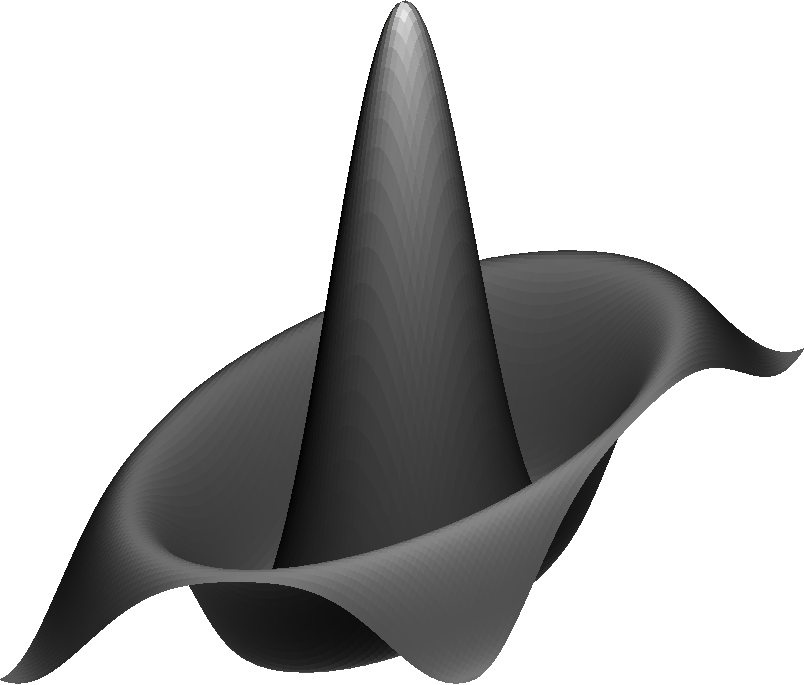
\includegraphics[scale=.4]{surfz}
\caption{An example of including the PDF graphics in the text ---
function $z=\frac{\sin(x^2+y^2)}{x^2+y^2}$}
\label{rys:surf}
\end{figure}


In this place I will omit the discussion
of the details of the graphics conversion to the PDF format ---
I will only add that the majority of the graphical programs has a~feature
of saving a~file to this format, which constitutes the universal graphics format.
An alternative for the PDF format, especially with reference to bitmaps
(photographs, scans, screenshots) is the PNG format, which is recommended
while creating CS articles.

A package, thanks to which we can place graphics in the \LaTeX
document, is the \verb|graphicx| one. In addition, it enables
some operations on the included graphics, such as: scaling, rotation,
mirror image, cropping, figure's ,,point of view'' change etc.
(details are available in the documentation of the package TeXLive,
catalogue \verb|\texmf\doc|\allowbreak\verb|\latex\graphics\|).

There is another kind of graphics presented
in the figure \ref{rys:2} (file \verb|schem01.1|)
and below there is a~printout of the \TeX source fragment,
illustrating a~method of including this illustration in a~document:
%
\begin{listing}[1]{1}
\begin{figure}[!htb]
  \centering
  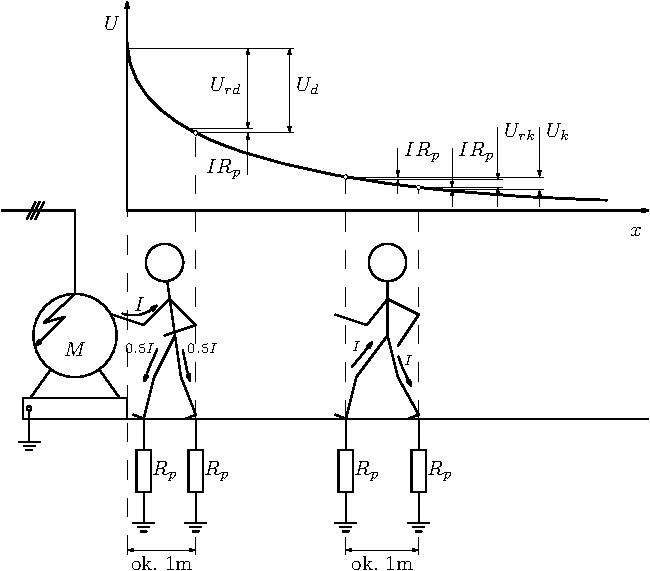
\includegraphics[scale=.7]{schem01}
  \caption{Outline illustrating a~phenomenon of the ,,step voltage''}
  \label{rys:2}
\end{figure}
\end{listing}

\begin{figure}[!htb]
  \centering
  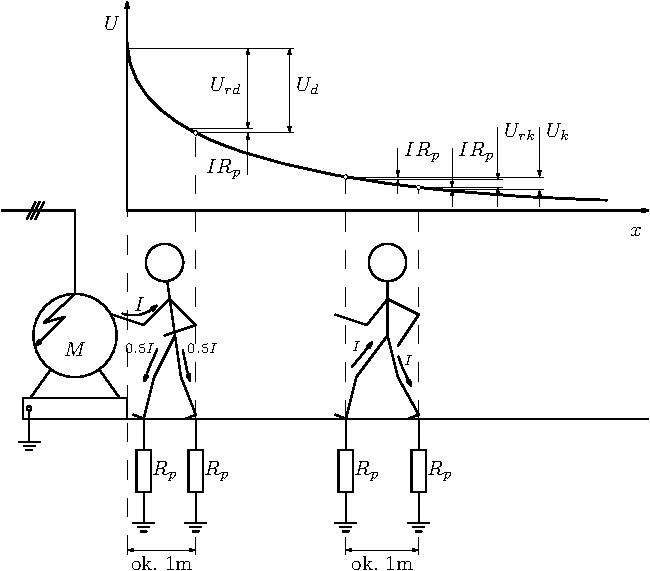
\includegraphics[scale=.7]{schem01}
  \caption{Outline illustrating a~phenomenon of the ,,step voltage''}
  \label{rys:2}
\end{figure}

Thanks to the usage of the \verb|tabular| environment, we have the
possibility of assembly several graphics on one area of the \verb|figure|
type, as it is illustrated in the figure \ref{rys:2szt}.

\begin{listing}[1]{1}
\begin{figure}[!htb]
\centering
  \begin{tabular}{*2{r@{\hskip4pt}l}}
  a)&&b)&\\[-10pt]
  &\includegraphics[scale=.95]{thesefig.61}&
  &\includegraphics[scale=.95]{thesefig.62}
  \end{tabular}
  \caption{Courses registered in selected points
    of model circuit: a)~increasing signal; b)~sloping signal}
  \label{rys:2szt}
\end{figure}
\end{listing}

\begin{figure}[!hb]
\centering
  \begin{tabular}{*2{r@{\hskip4pt}l}}
  a)&&b)&\\[-10pt]
  &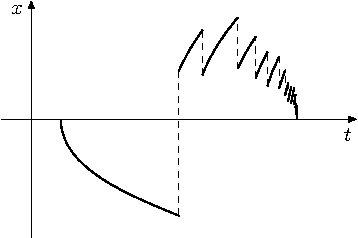
\includegraphics[scale=.95]{thesefig61}&
  &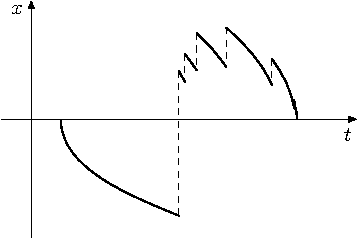
\includegraphics[scale=.95]{thesefig62}
  \end{tabular}
  \caption{Courses registered in selected points
    of model circuit: a)~increasing signal; b)~sloping signal}
  \label{rys:2szt}
\end{figure}

\subsection{A few words more about the graphics}
As it was mentioned earlier --- ,,PDF is unequal to PDF'',
apart from the aspects of the incompatibility with the standards
of various \textit{drivers} --- essential thing is the proper
preparation of the graphics for the target paper printed
with the offset technique.

If we make the graphics in the program that uses the vector technique,
we have to remember about proper diversification of line thickness.
One should beware of the settings of the ,,hair thickness'' type,
as actually it assigns one-pixel thickness to a~stroke.
Therefore, in fact the thickness of a~stroke would depend on
the resolution of a~print device. The larger resolution,
the thinner stroke\dots{} The thickness of strokes should be
defined in the absolute units, i.e. 0,4\,pt.

If the graphics comes from a~program to bitmaps processing (i.e.
scanned illustrations) --- one should pay attention to appropriate
quality of such a~graphics: readability, contrast, lack of pale colors
of the background, legible descriptions. It may happen that such an illustration
would require some extra work in the form of the retouch or making new, more
clear\vadjust{\goodbreak}text descriptions. The minimal advisable resolution
of such bitmaps is 600\,dpi for black and white \textit{art-line} illustrations
or 300\,dpi for black and white \textit{grayscale} illustration or colourful illustrations.


\section{Guidelines of the AGH Publishing House concerning the literature}

In the publication \cite{UWND-AGH} there are rules
related to the order of the bibliographic entry
applied by the AGH Publishers. Present point, together with
the examples, has been taken from this publication.

In case of books, one is supposed to provide the following data:
%
\begin{itemize}
\item Author's surname
\item initial/initials of author's name/names
\item book's title -- in italics
\item publication's number
\item a~place of the publication
\item publisher
\item the year of the publication
\item ISBN number (if it is provided)
\end{itemize}

For example:
%[1] Billingsley P.:
%\textit{Probability and measure}. New York, John Wiley 1979
[1] Giesecke F.\,E. \textit{et al.}:
\textit{Engineering Graphics}.
3rd ed with Computer Graphics.
New York, Macmillan Publishing Co., Inc. 1985,
ISBN~0-02-342650-0


\medskip

An order of the bibliographic entry used by the AGH Publishers
for periodicals is as follows:
%
\begin{itemize}
\item Author's surname
\item initial/initials of author's name/names
\item article's title -- in italics
\item journal's title
\item number
\item the year of the publication
\item pages from--to
\end{itemize}


For example:
[2] Briggs F.:
\textit{On problems of estimation in Leontief models}.
Econometrica, vol. 25, 1957, 444--455

\medskip

An order of the bibliographic entry used by the AGH Publishers
for the conference materials is as follows:
%
\begin{itemize}
\item Author's surname
\item initial/initials of author's name/names
\item article's/paper's title -- in italics
\item $[$in:$]$
\item conference's name
\item conference's place and date
\end{itemize}

For example:
[3] Gaj�cki M.:
\emph{Automatyczne generowanie s�ownika
asocjacyjnego na podstawie korpusu tekst�w}.
[in:]
V Krajowa Konferencja Naukowa ,,In�ynieria Wiedzy i Systemy Ekspertowe'',
Wroc�aw 2003

The easiest way of proper formatting of the bibliography is to use the predefined .BST with BiBTeX.



\section{How should the author's submission look like?}

As a~result of the compilation with the use of the \texttt{csagh.sty} style,
we obtain a~setting of the article without the live pagination and without
the final pages numbering. These setting's elements will be made during
the preparation for the print of the current ,,Computer Science'' issue.
Therefore, if we use the automatic references -- we do not provide a~page number,
which, in the final version of the CS publication, may be completely different than
in the current article, composed as a~draft. References should concern the numbers of
the document's logical structures: subsection, number of an equation, theorem, figure,
table etc.

In a~draft version, at the bottom of the page there are printed only the current
date of the last document compilation and the information about the amount of the
pages printed (the number of a~current page and the total amount of pages).

%The author is obliged to send two copies of the article printout (together with the
%figures) to the address of the selected member of the Annual's Editorial Committee.
%
%One should attach to the paper:
%\begin{itemize}
%\item a~digital version with complete \TeX sources
			%and used graphics and compiled version as well
      %(PostScript or PDF);
%\item a~statement, signed by the Author, of text originality and readiness for
			%the article correction demanded by the Reviewer.
%\end{itemize}
%
%The required set may be sent to the e-mail address:
%\texttt{zncs@icsr.agh.edu.pl}.

The author should use the OJS Submission System \url{http://journals.agh.edu.pl/csci} to
send the compiled version of the manuscript (PDF) and after revision, the source files (ZIP).
Please mind that the figures should be of a good quality (we prefer monochrome versions of figures,
especially for different schemes).

The Authors will be asked for realization of the author's correction of the setting and to 
follow the guidelines of the statistical and language correctors.

\begin{acknowledgements}
  This is the place for a~list of the acknowledgements for sponsors,
	donors, benefactors and all the people of goodwill, which contributed
	to as essential as the financial support of the subject matter of the
	issue raised in the article\dots{} Certainly, if someone
  has such a~will or wish, or else another commitments.
	There is also placed information about grants or grants-in-aid.

  For my part, I offer thanks to \TeX creator, professor
  Donald E. Knuth for creation of such a~perfect tool.
\end{acknowledgements}

\nocite{*}

\bibliographystyle{cs-agh}
\bibliography{bibliography}

\end{document}

% -*- TeX:PL -*-
